\documentclass[@BEAMER_OPTIONS@]{beamer}
    @USE_PGFPAGES@

    \usetheme[alternativetitlepage=true,titleline=true]{Torino}
    \setbeamertemplate{navigation symbols}{}
    \setbeamertemplate{note page}[plain]
    \setbeamertemplate{caption}{\insertcaption}


    \usepackage[utf8]{inputenc}
    \usepackage[russian]{babel}
    \usepackage{graphicx}
    \usepackage{subfigure}
    \usepackage{xspace}
    \usepackage{adjustbox}
    \usepackage{tikz}
    \usepackage{relsize}
    \usepackage{fancyvrb}
    \fvset{fontsize=\footnotesize}
    \RecustomVerbatimEnvironment{verbatim}{Verbatim}{}
    \usepgflibrary{arrows}
    \usetikzlibrary{shadows,decorations.pathreplacing,patterns,shapes}
    \tikzstyle{every picture}=[semithick,>=stealth,remember picture]
    \usepackage{inconsolata}
    \usepackage{listings}
    \lstset{
        language=C++,
        basicstyle=\footnotesize\rmfamily,
        keywordstyle=\color{chameleon1}\bfseries,
        commentstyle=\color{chameleon4}\it\rmfamily,
        stringstyle=\color{chameleon4},
        numbers=left,
        numberstyle=\tiny,
        aboveskip=-0.02\baselineskip,
        belowskip=-0.02\baselineskip,
        columns=flexible,
        extendedchars=false,
        showstringspaces=false,
        morekeywords={global,kernel,ulong,size_t,cl_uint,cl_platform_id}
        }
    \newcommand{\code}[1]{\lstinline|#1|}
    \protected\def\plusplus{{\nolinebreak[4]\hspace{-.05em}\raisebox{.4ex}{\relsize{-3}\bf ++}}\xspace}
    \newcommand{\CXX}{{\rm C}\plusplus}
    \newcommand{\CC}{{\rm C99}\xspace}
    \newcommand{\www}[1]{\href{#1}{#1}}

    \usepackage{ifthen}
\usetikzlibrary{shadows.blur}
\newlength{\ribbonoffset}
\setlength{\ribbonoffset}{3em}

% corner, color, text
\newcommand{\ribbon}[3]{
  \ifthenelse{\equal{#1}{east}}{%
    \tikzset{ribbonrot/.style={rotate=-45}}
  }{%
    \tikzset{ribbonrot/.style={rotate=45}}
  }
  \begin{tikzpicture}[remember picture, overlay]
    \node[ribbonrot, shift={(0, -\ribbonoffset)}] at (current page.north #1) {
      \begin{tikzpicture}[remember picture, overlay,scale=0.5]
        \node[
            fill=#2,
            text centered,
            minimum width=50em,
            minimum height=1.2em,
            blur shadow,
            shadow yshift=0pt,
            shadow xshift=0pt,
            shadow blur radius=.2em,
            shadow opacity=50,
            text=white
            ](fmogh) at (0pt, 0pt) {%
            \fontfamily{phv}\selectfont\bfseries\tiny#3};
        \draw[
            white,
            dashed,
            line width=.04em,
            dash pattern=on .2em off 1.5\pgflinewidth
            ] (-25em,1em) rectangle (25em,-1em);
      \end{tikzpicture}
    };
  \end{tikzpicture}
}

    \newcommand{\forkme}{\ribbon{east}{chameleon1}{white}{\href{https://github.com/ddemidov/vexcl}{Fork me on GitHub}}}
    \newcommand{\singledevice}{\ribbon{east}{chameleon2}{chameleon4}{Одно устройство}}

    \tikzset{
        treenode/.style={
            draw,
            fill=white,
            blur shadow,
            shadow xshift=1pt,
            shadow yshift=-1pt,
            shadow blur radius=2pt,
            shadow opacity=40
            }
        }


    \title{VexCL}
    \subtitle{библиотека векторных выражений для OpenCL/CUDA}
    \author{Денис Демидов}
    \institute{
        Казанский Федеральный Университет\\
        Институт системных исследований РАН
    }
    \date{21.04.2016}

\begin{document}

%----------------------------------------------------------------------------
\begin{frame}{}
    \titlepage
\end{frame}

%----------------------------------------------------------------------------
\section{VexCL}

%----------------------------------------------------------------------------
\begin{frame}{VexCL~--- библиотека векторных выражений для OpenCL/CUDA}
    \forkme
    \begin{itemize}
        \item Создана для облегчения разработки GPGPU приложений на \CXX
            \begin{itemize}
                \item Удобная нотация для векторных выражений
                \item Автоматическая генерация ядер OpenCL/CUDA во время
                    выполнения
            \end{itemize}
            \vspace{\baselineskip}
        \item Поддерживаемые технологии
            \begin{itemize}
                \item OpenCL (Khronos \CXX API, Boost.Compute)
                \item NVIDIA CUDA
            \end{itemize}
            \vspace{\baselineskip}
        \item Исходный код доступен под лицензией MIT
    \end{itemize}
\end{frame}

\note[itemize]{
\item VexCL is a vector expression template library for OpenCL. It allows you
    to use convenient matlab-like notation for vector operations and it
    generates the appropriate compute kernels for you automatically.
\item The library is header-only, so you don't have to build it to use it. The
    source code of the library is available on GitHub under very liberal
    MIT license.
}

%----------------------------------------------------------------------------
\begin{frame}[fragile]{Hello VexCL: vector sum}
    \vspace{-1\baselineskip}
    \begin{columns}
        \begin{column}{0.2\textwidth}
            \begin{minipage}[c][\textheight][c]{\linewidth}
                \begin{exampleblock}{OpenCL}
                    \begin{adjustbox}{width=0.19\textwidth, height=\textheight, keepaspectratio}
                        \begin{minipage}{\textwidth}
                            \lstinputlisting[linerange={1-72}]{code/hello-opencl.cpp}
                        \end{minipage}
                    \end{adjustbox}
                \end{exampleblock}
            \end{minipage}
        \end{column}
        \begin{column}{0.7\textwidth}
            \begin{minipage}[c][\textheight][c]{\linewidth}
                \begin{exampleblock}{VexCL}
                    \begin{adjustbox}{width=0.7\textwidth, height=\textheight, keepaspectratio}
                        \begin{minipage}{\textwidth}
                            \lstinputlisting[linerange={1-19}]{code/hello-vexcl.cpp}
                        \end{minipage}
                    \end{adjustbox}
                \end{exampleblock}
            \end{minipage}
        \end{column}
    \end{columns}
\end{frame}

\note[itemize]{
\item Here is the simplest example of using vexcl: addition of two vectors on a
    gpu card.
\item The first line is the context initialization. We provide a device filter
    to the context constructor and get all compute devices that satisfy the
    filter. Here we filter by type and get all available GPUs.
\item Data allocation and transfer is also simplified. \code{vex::vector}
    constructor allocates memory on device and possibly transfers initial data
    as well. The parameters here are list of command queues and either size or
    input host vector.
\item Line ten does what's needs to be done here. This simple expression leads
    to automatic kernel generation and launch. And then we copy the results
    back to host and see what we got.
}

%----------------------------------------------------------------------------
\begin{frame}[fragile]{Вычислительные ядра генерируются автоматически}
    \begin{columns}
        \begin{column}{0.38\textwidth}
            \begin{exampleblock}{Выражение:}
                \begin{lstlisting}
x = 2 * y - sin(z);
                \end{lstlisting}
            \end{exampleblock}
        \end{column}
        \begin{column}{0.55\textwidth}
            \begin{itemize}
                \item \code{export VEXCL_SHOW_KERNELS=1}\\
                    чтобы увидеть сгенерированный код.
            \end{itemize}
        \end{column}
    \end{columns}
    \begin{exampleblock}{Ядро:}
        \begin{lstlisting}
kernel void vexcl_vector_kernel(
    ulong n,
    global double * prm_1,
    int prm_2,
    global double * prm_3,
    global double * prm_4
)
{
    for(size_t idx = get_global_id(0); idx < n; idx += get_global_size(0)) {
        prm_1[idx] = ( ( prm_2 * prm_3[idx] ) - sin( prm_4[idx] ) );
    }
}
        \end{lstlisting}
    \end{exampleblock}
    \begin{tikzpicture}[overlay,scale=0.6]
        \draw (16,8) node(sub)[draw,fill=white,ellipse,drop shadow]{$-$};

        \draw (sub) +(-2.00,-1) node(mul)[draw,fill=white,drop shadow,ellipse]{$*$};
        \draw (sub) +( 2.00,-1) node(sin)[draw,fill=white,drop shadow,ellipse]{sin};
        \draw (mul) +(-2.00,-1) node(two)[draw,fill=white,drop shadow,minimum size=0.5cm]{2};
        \draw (mul) +( 2.00,-1) node(y)  [draw,fill=white,drop shadow,minimum size=0.5cm]{y};
        \draw (sin) +( 1.75,-1) node(z)  [draw,fill=white,drop shadow,minimum size=0.5cm]{z};

        \draw (sub) -- (mul);
        \draw (sub) -- (sin);
        \draw (mul) -- (two);
        \draw (mul) -- (y);
        \draw (sin) -- (z);
    \end{tikzpicture}
\end{frame}

%----------------------------------------------------------------------------
\begin{frame}[fragile]{Язык векторных выражений VexCL}
    \begin{columns}
        \begin{column}{0.4\textwidth}
            \begin{itemize}
                \item Векторы, скаляры, константы
                \item Арифм. и логич. операторы
                \item Встроенные функции
                \item Пользовательские функции
                \item Генераторы случайных чисел
                \item Сортировка, префиксные суммы
            \end{itemize}
        \end{column}
                \begin{column}{0.4\textwidth}
                    \begin{itemize}
                        \item Временные значения
                        \item Срезы и перестановки
                        \item Редукция (сумма, экстремумы)
                        \item Произв. матрицы на вектор
                        \item Свертки
                        \item Быстрое преобразование Фурье
                    \end{itemize}
                \end{column}
    \end{columns}
\end{frame}

\note[itemize]{
\item So, what kind of expressions can you use in VexCL?
\item First, any vectors used in an expression have to be compatible.
\item If this requirement is satisfied, then expressions may combine
    vectors and scalars with almost any binary operators. OpenCL math functions
    and user-defined functions are also available.
}

%----------------------------------------------------------------------------
\begin{frame}[fragile]{Пример: оценка числа $\pi$ методом Монте-Карло}
    \vspace{-1\baselineskip}
    \begin{columns}
        \begin{column}{0.55\textwidth}
            \begin{itemize}
                \item Приближенная оценка $\pi$:
            \end{itemize}
            \vspace{\baselineskip}
            \begin{equation*}
                \frac{\text{площадь круга}}{\text{площадь квадрата}} =
                \frac{\pi r^2}{(2r)^2} = \frac{\pi}{4},
            \end{equation*}
            \begin{equation*}
                \pi = 4 \frac{\text{площадь круга}}{\text{площадь квадрата}}
                \approx 4 \frac{\text{\color{chameleon4}{точки в
                круге}}}{\text{\color{chameleon4}{все}
                \color{chameleon1}{точки}}}
            \end{equation*}
        \end{column}
        \begin{column}{0.35\textwidth}
            \begin{figure}
                \includegraphics[width=\textwidth]{mcpi}
            \end{figure}
        \end{column}
    \end{columns}
    \begin{exampleblock}{}
        \begin{lstlisting}[texcl=true]
vex::Random<cl_double2> rnd;
vex::Reductor<size_t, vex::SUM> sum(ctx);

double pi = 4.0 * sum( length( rnd(vex::element_index(0, n), seed) ) < 1 ) / n;
        \end{lstlisting}
    \end{exampleblock}
\end{frame}

\note[itemize]{
\item Here is a bit more complex example of what you can do with VexCL.
\item Imagine we want to compute an approximate value of $\pi$ with Monte-Carlo
    method. We can use the following equalities to do this.
}

%----------------------------------------------------------------------------
\begin{frame}[fragile]{Монте-Карло $\pi$: сгенерированное ядро}
    \begin{columns}
        \begin{column}[t]{0.2\textwidth}
            \begin{exampleblock}{}
                \begin{adjustbox}{width=0.23\textwidth, height=\textheight, keepaspectratio}
                    \begin{minipage}{\textwidth}
                        \lstinputlisting[linerange={1-49}]{code/pi-kernel.cpp}
                    \end{minipage}
                \end{adjustbox}
            \end{exampleblock}
        \end{column}
        \begin{column}[t]{0.2\textwidth}
            \begin{exampleblock}{}
                \begin{adjustbox}{width=0.23\textwidth, height=\textheight, keepaspectratio}
                    \begin{minipage}{\textwidth}
                        \lstinputlisting[firstnumber=last,linerange={50-98}]{code/pi-kernel.cpp}
                    \end{minipage}
                \end{adjustbox}
            \end{exampleblock}
        \end{column}
        \begin{column}[t]{0.2\textwidth}
            \begin{exampleblock}{}
                \begin{adjustbox}{width=0.23\textwidth, height=\textheight, keepaspectratio}
                    \begin{minipage}{\textwidth}
                        \lstinputlisting[firstnumber=last,linerange={99-147}]{code/pi-kernel.cpp}
                    \end{minipage}
                \end{adjustbox}
            \end{exampleblock}
        \end{column}
        \begin{column}[t]{0.3\textwidth}
            \begin{exampleblock}{}
                \begin{adjustbox}{width=0.23\textwidth, height=\textheight, keepaspectratio}
                    \begin{minipage}{\textwidth}
                        \lstinputlisting[firstnumber=last,linerange={148-196}]{code/pi-kernel.cpp}
                        \vspace{\baselineskip}
                    \end{minipage}
                \end{adjustbox}
            \end{exampleblock}
        \end{column}
    \end{columns}
\end{frame}

%----------------------------------------------------------------------------
\section{Примеры использования}

\begin{frame}
    \sectionpage
\end{frame}

\begin{frame}{Геофизические расчеты}
    \begin{columns}
        \begin{column}{0.45\textwidth}
            \begin{itemize}
                \item ЗАО <<Градиент>>~--- Казанская геофизическая компания,
                    выполняющая микросейсмические исследования с целью оценки
                    нефтегазоносности геологических объектов.
                \item Гетерогенный вычислительный кластер занимает 38 место в
                    Top50 по России
                \item Для ускорения расчетов используется VexCL
            \end{itemize}
        \end{column}
        \begin{column}{0.55\textwidth}
            \begin{figure}
                \includegraphics[width=\textwidth]{microseism}
            \end{figure}
        \end{column}
    \end{columns}
\end{frame}

\begin{frame}{Boost.odeint~--- библиотека численного интегрирования ОДУ}
    \begin{columns}
        \begin{column}{0.65\textwidth}
            \begin{itemize}
                \item Позволяет эффективно проводить параметрические
                    исследования ОДУ на GPU с помощью VexCL.
                \item[{[1]}] D. Demidov, K. Ahnert, K. Rupp, and P. Gottschling.\\
                    Programming CUDA and OpenCL: A Case Study Using Modern \CXX Libraries.\\
                    \emph{SIAM J. Sci. Comput.,} 35(5):C453 – C472, 2013.\\
                    \href{http://dx.doi.org/10.1137/120903683}{doi:10.1137/120903683}
                \item[{[2]}] K. Ahnert, D. Demidov, and M. Mulansky.\\
                    Solving ordinary differential equations on GPUs.\\
                    In \emph{Numerical Computations with GPUs} (pp. 125-157).  Springer, 2014.
                    \href{http://dx.doi.org/10.1007/978-3-319-06548-9\_7}{doi:10.1007/978-3-319-06548-9\_7}
            \end{itemize}
        \end{column}
        \begin{column}{0.35\textwidth}
            \begin{figure}
                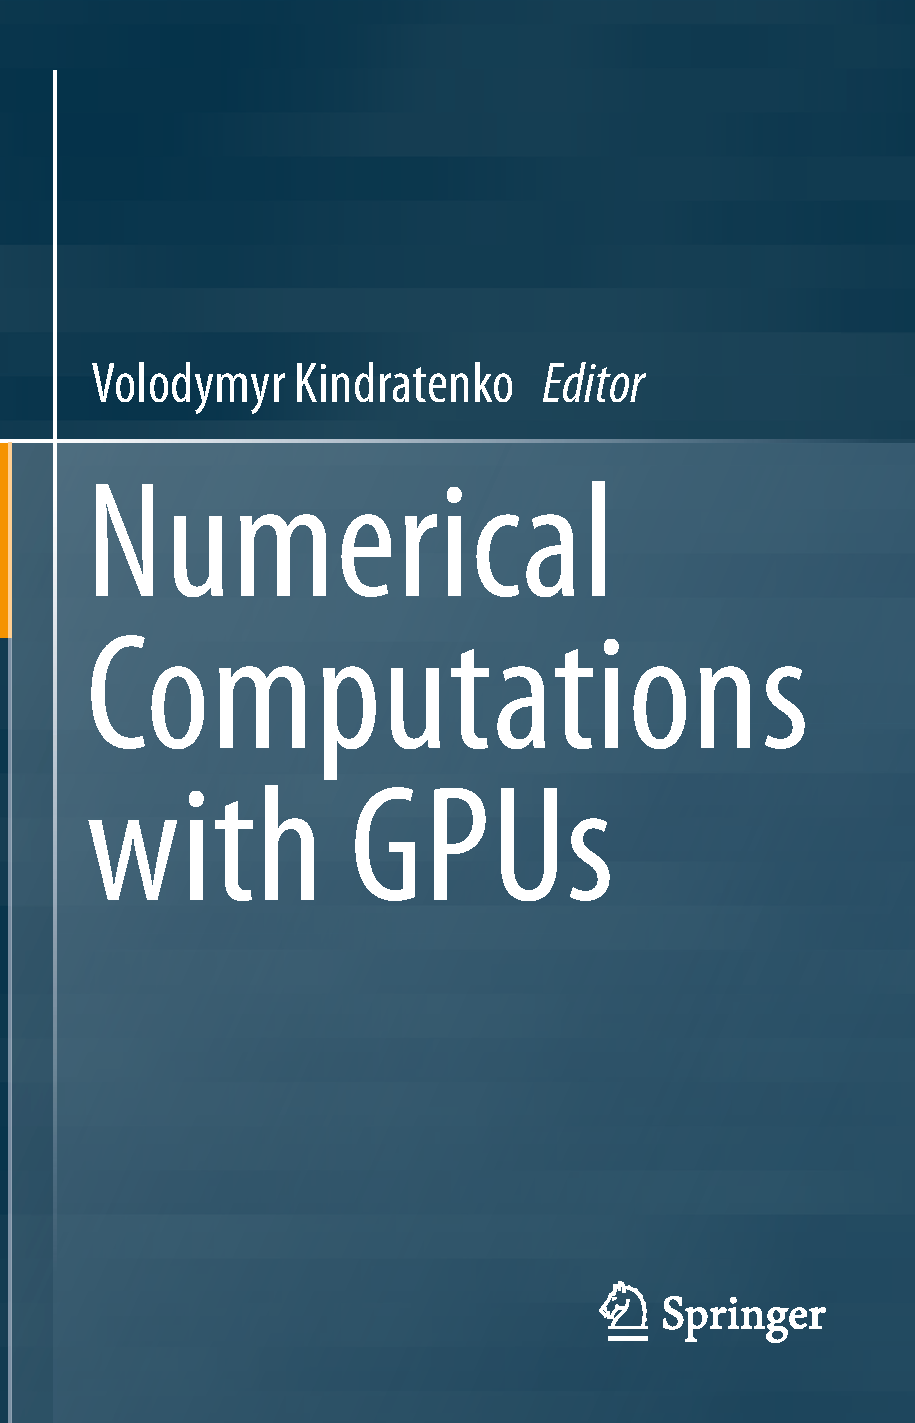
\includegraphics[height=0.8\textheight]{ncwg}
            \end{figure}
        \end{column}
    \end{columns}
\end{frame}

\begin{frame}{Шумоподавляющие фильтры для растровых изображений}
    \begin{columns}
        \begin{column}{0.4\textwidth}
            \begin{itemize}
                \item Pascal Schmitt, Georg-Augustus-Universit\"at,
                    G\"ottingen, Germany
                \item Ускорение~--- до 20x по сравнению с CPU
                \item Реализовал преобразование Фурье и генерацию случайных
                    чисел в VexCL
            \end{itemize}
        \end{column}
        \begin{column}{0.55\textwidth}
            \vspace{-1\baselineskip}
            \begin{figure}
                \only<1>{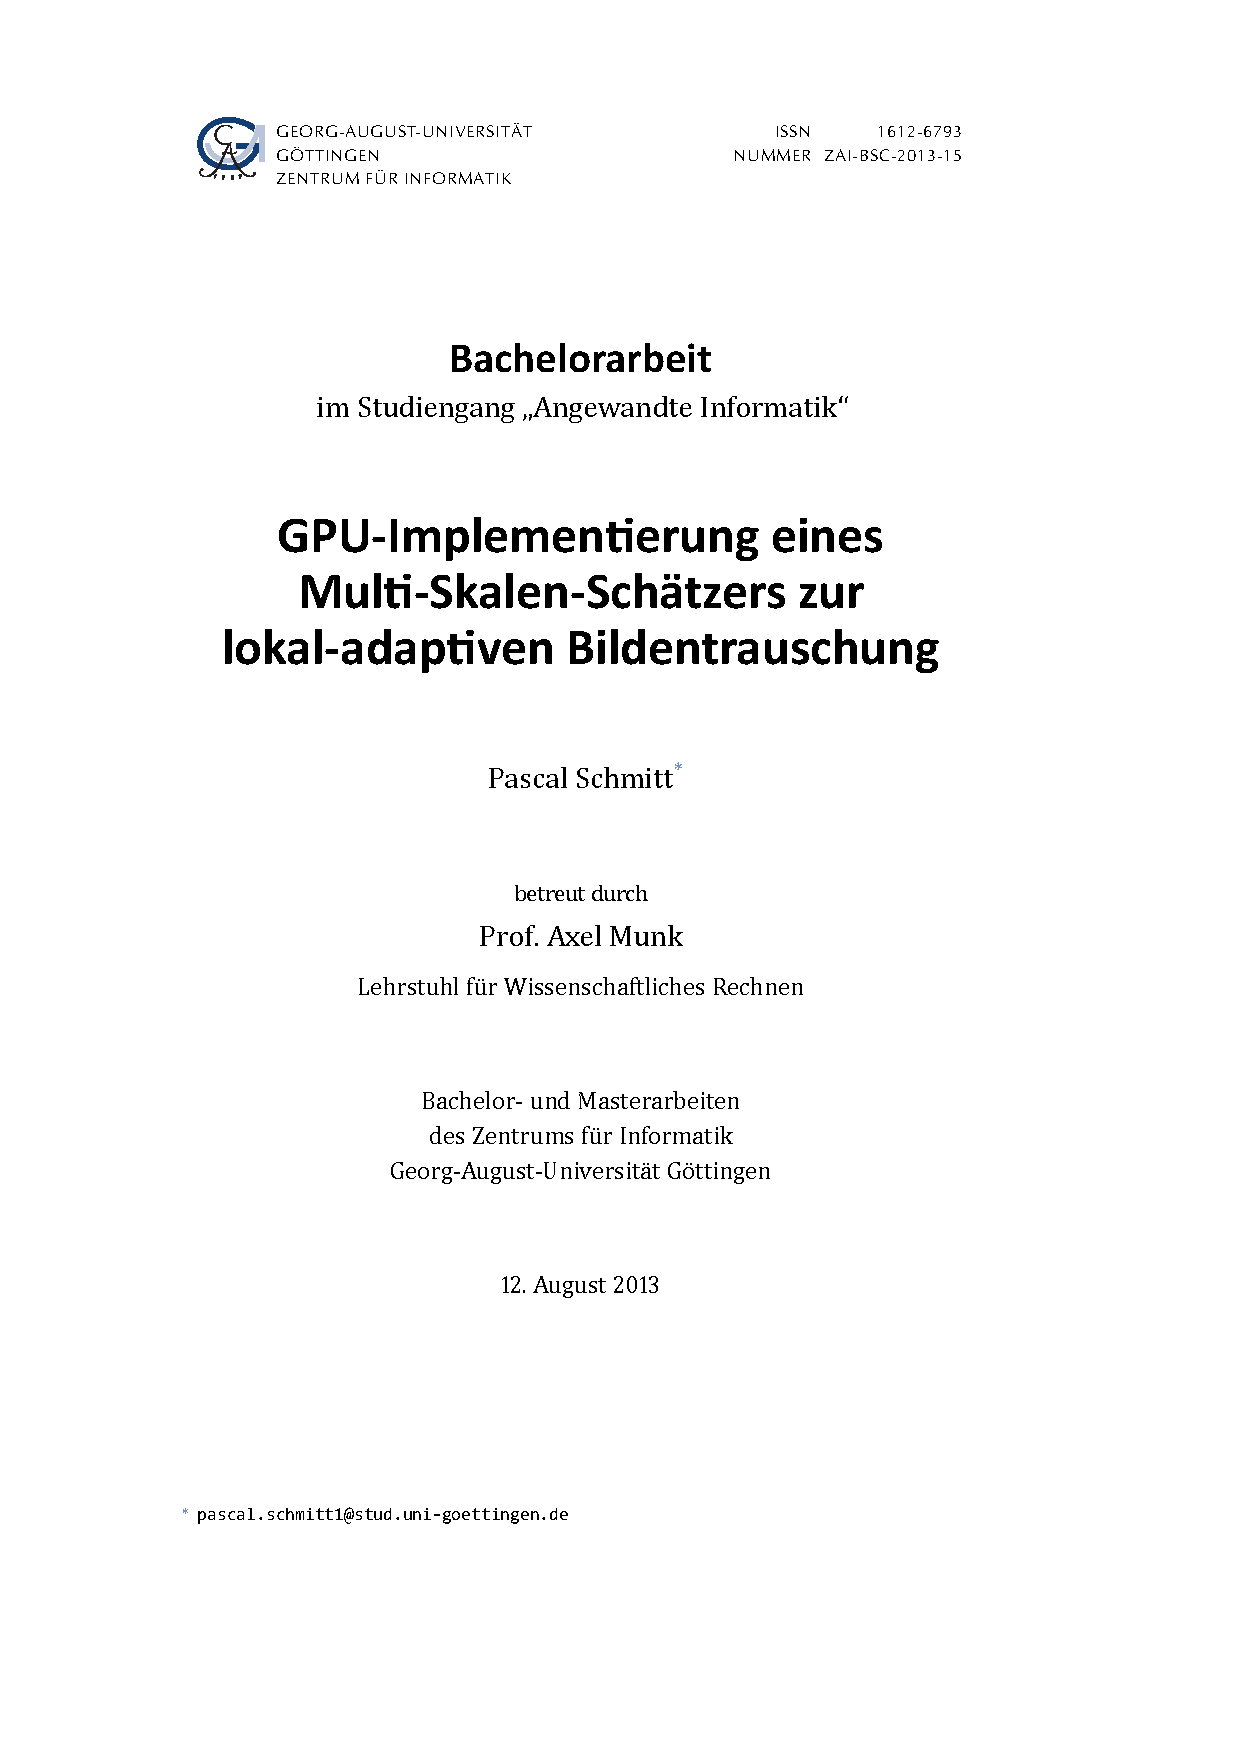
\includegraphics[height=\textheight]{neapel-1}}%
                \only<2>{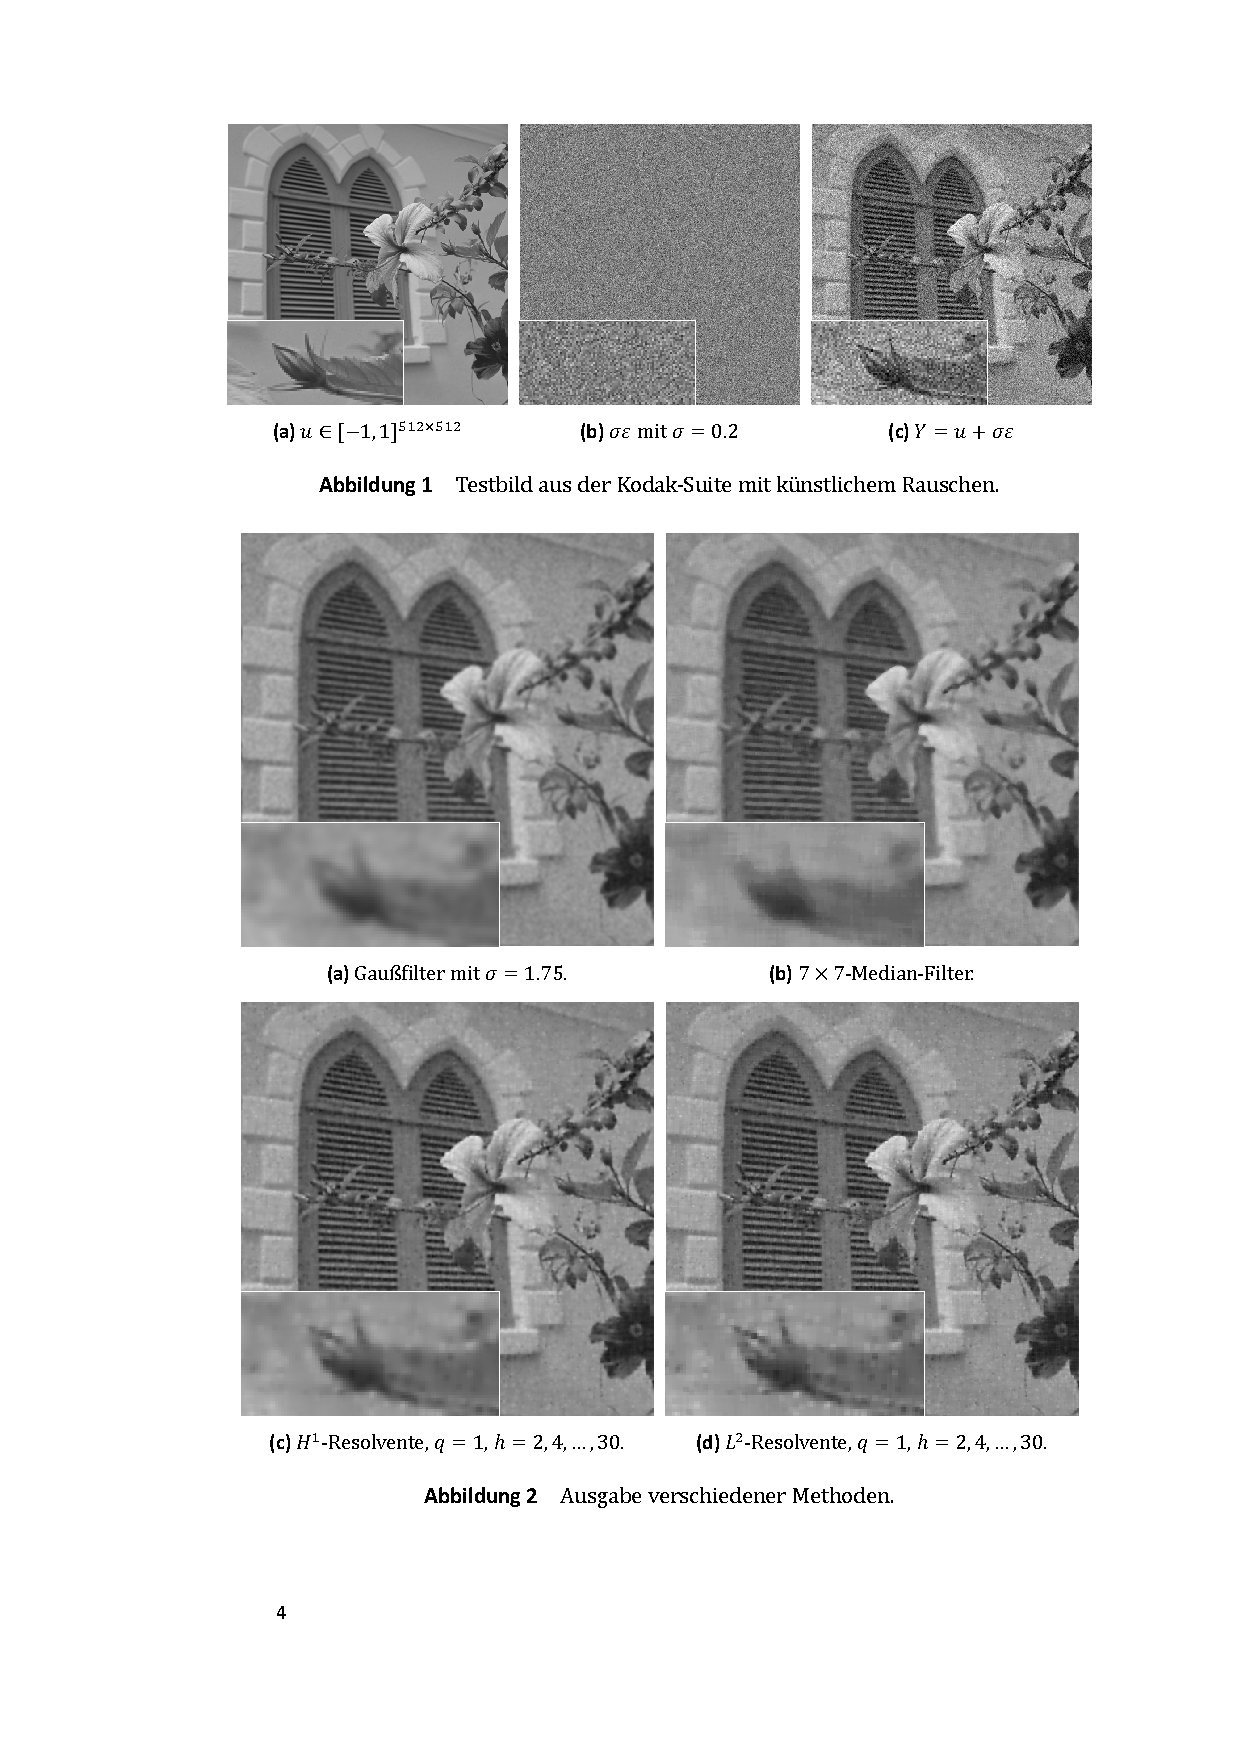
\includegraphics[height=\textheight]{neapel-2}}
            \end{figure}
        \end{column}
    \end{columns}
\end{frame}

\begin{frame}{Antioch}{A New Templated Implementation Of Chemistry for Hydrodynamics}
    \begin{columns}
        \begin{column}{0.5\textwidth}
            \begin{itemize}
                \item University of Texas at Austin, USA
                \item \www{https://github.com/libantioch/antioch}
                \item Гидродинамические расчеты с учетом химических реакций
                \item Для расчетов на GPU используется VexCL
            \end{itemize}
        \end{column}
        \begin{column}{0.5\textwidth}
            \begin{figure}
                \only<1>{\includegraphics[width=\textwidth]{antioch-1}}%
                \only<2>{\includegraphics[width=\textwidth]{antioch-2}}
            \end{figure}
        \end{column}
    \end{columns}
\end{frame}

\begin{frame}{Оценка положения судна в пространстве}
    \begin{columns}
        \begin{column}{0.5\textwidth}
            \vspace{-2\baselineskip}
            \begin{figure}
                \includegraphics[width=0.8\textwidth]{ship-channel}
            \end{figure}
            \begin{itemize}
                \item University of Antwerp, Belgium
                \item Обработка данных лидара в реальном времени с помощью GPU
                \item Ускорение~--- 1000x по сравнению с примитивным алгоритмом
                    на CPU
            \end{itemize}
        \end{column}
        \begin{column}{0.45\textwidth}
            \vspace{-3\baselineskip}
            \begin{figure}
                \includegraphics[height=1.05\textheight]{smidt}
            \end{figure}
        \end{column}
    \end{columns}
\end{frame}

\begin{frame}{Решение разреженных СЛАУ большой размерности}
    \begin{itemize}
        \item Реализация алгебраического многосеточного метода
        \item \www{https://github.com/ddemidov/amgcl}
        \item Для ускорения расчетов на GPU используется VexCL
    \end{itemize}
\end{frame}

\begin{frame}{Kratos Multi-Physics}
    \begin{columns}
        \begin{column}{0.45\textwidth}
            \begin{itemize}
                \item International Center for Numerical Methods in
                    Engineering, Barcelona, Spain
                \item \www{http://www.cimne.com/kratos/}
                \item Пакет с открытым исходным кодом для инженерных расчетов
                \item В качестве решателя по умолчанию используется AMGCL
            \end{itemize}
        \end{column}
        \begin{column}{0.55\textwidth}
            \begin{figure}
                \includegraphics[width=\textwidth]{kratos}
            \end{figure}
        \end{column}
    \end{columns}
\end{frame}

%----------------------------------------------------------------------------
\begin{frame}[fragile]{}
    \begin{itemize}
        \item VexCL позволяет писать компактный и читаемый код
            \begin{itemize}
                \item Хорошо подходит для быстрой разработки научных GPGPU
                    приложений.
                \item Производительность часто сравнима с ядрами, написанными
                    вручную.
            \end{itemize}
            \vspace{\baselineskip}
            \item[{[1]}] D. Demidov, K. Ahnert, K. Rupp, and P. Gottschling.\\
                Programming CUDA and OpenCL: A Case Study Using Modern \CXX Libraries.\\
                \emph{SIAM J. Sci. Comput.,} 35(5):C453 – C472, 2013.\\
                \href{http://dx.doi.org/10.1137/120903683}{doi:10.1137/120903683}
            \item[{[2]}] K. Ahnert, D. Demidov, and M. Mulansky.\\
                Solving ordinary differential equations on GPUs.\\
                In \emph{Numerical Computations with GPUs} (pp. 125-157).  Springer, 2014.
                \href{http://dx.doi.org/10.1007/978-3-319-06548-9\_7}{doi:10.1007/978-3-319-06548-9\_7}
    \end{itemize}
\end{frame}

\end{document}
